\documentclass[11pt,psfig]{article}
\usepackage{epsfig}
\usepackage{times}
\usepackage{amssymb}
\usepackage{float}

\newcount\refno\refno=1
\def\ref{\the\refno \global\advance\refno by 1}
\def\ux{\underline{x}}
\def\uw{\underline{w}}
\def\bw{\underline{w}}
\def\ut{\underline{\theta}}
\def\umu{\underline{\mu}} 
\def\bmu{\underline{\mu}} 
\def\be{p_e^*}
\newcount\eqnumber\eqnumber=1
\def\eq{\the \eqnumber \global\advance\eqnumber by 1}
\def\eqs{\eq}
\def\eqn{\eqno(\eq)}

 \pagestyle{empty}
\def\baselinestretch{1.1}
\topmargin1in \headsep0.3in
\topmargin0in \oddsidemargin0in \textwidth6.5in \textheight8.5in
\begin{document}
\setlength{\parskip}{1.2ex plus0.3ex minus 0.3ex}


\thispagestyle{empty} \pagestyle{myheadings} \markright{G}



\title{CS 266, Computational Geometry, Homework 1}
\author{Zachary DeStefano, PhD student, 15247592}
\date{Due Date: April 10, 2014}

\maketitle

\vfill\eject

\section*{Problem 1.6}

\subsection*{Problem 1.6 Part A}

Since the convex hull is a convex set containing all the points, if we take the convex hull of the 2n endpoints, then by convexity, all the line segments will be in the hull. 
\\
\\
Since the endpoints are on the line, a convex set of the n line segments must contain all the 2n endpoints. Since the convex hull of 2n endpoints is the smallest convex set that contains all the endpoints, it is thus the smallest convex set that contains all the n line segments, thus it is the convex hull of the line segments. 

\subsection*{Problem 1.6 Part B}

Let P be a non-convex polygon. Algorithm for finding the convex hull of P in O(n) time:
\\
1. Find left-most point and right-most point in polygon, call them $p_1$ and $q_1$. \\
2. Let $p_1,...,p_n$ be the points from $p_1$ to $q_1$ in clockwise order in the polygon and let $p_n=q_1$. \\
3. To compute the upper hull, follow steps 3-6 of the ConvexHull algorithm in section 1.1 for the points $p_1,...,p_n$ however in step 5, add the condition that the x-coordinate needs to increase in addition to the last three points making a right turn.\\
4. Let $q_1,...,q_n$ be the points from $q_1$ to $p_1$ in clockwise order in the polygon and let $q_n=p_1$. \\
5. To compute the lower hull, repeat step 3 but with the points $q_1,...,q_n$. The additional condition will be that the x-coordinate needs to decrease. 
\\
\\
Correctness:\\
At each step, we are both making a right turn and ensuring that the x-coordinate will increase, thus the convexity will be preserved. \\
We are only including points on the polygon in the algorithm thus we will get the smallest convex set. \\
\\
Run time:\\
Finding the left and right most points will take O(n) time.\\
The rest of the algorithm has the same run time as ConvexHull after the sorting, which is O(n).\\
Thus the algorithm takes O(n) time total.

\newpage


\section*{Problem 1.10}

\subsection*{Problem 1.10a}

Proof that the convex hull of S consists of straight lines and pieces of circles in S. 
\\
\\
Take a set of lines outside the area of the circles and move them toward the circles to make half-planes. The intersection of these half-planes will be a convex polygon that surrounds all the circles because we have a finite number of circles. \\
\begin{figure}[H]
\centering
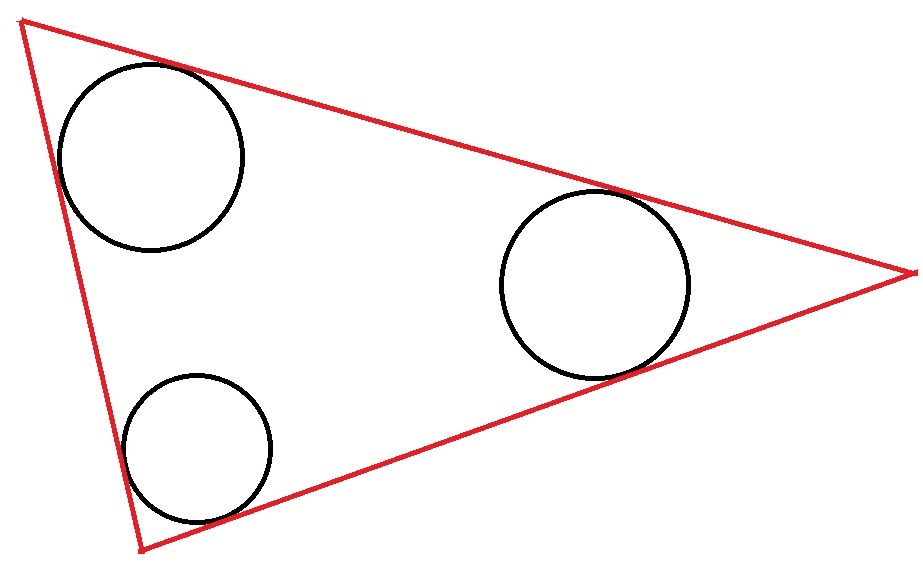
\includegraphics[height=4in]{hw1prob1-10a_1.jpg}
\caption{In black are the circles and in red is the convex polygon}
\end{figure}
In the corners of this polygon, there will be regions whose points do not need to be in the convex hull\\
In this case, the part of the hull will the arc formed in that corner instead of the corner itself. 
\\    This can be shown from the definition of hull as the intersection of all the half-planes with points in the hull. 
\\     If we form half-planes from the tangeants to the circle in this particular arc, then the intersection will definitely contain the circle. 
\\     It will only contain the circle:
\\					- Take point p outside circle and point c that is the center of the circle
\\					- Find the intersection of the circle with segment pc, call it q
\\					- Take the tangent line at q
\\					- The half-plane formed by it will contain the circle and not p
\begin{figure}[H]
\centering
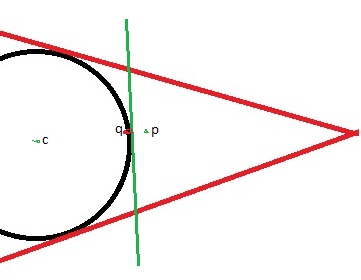
\includegraphics[height=2in]{hw1prob1-10a_2.jpg}
\caption{The points p,q,c illustrated by zooming in on the left part of the above figure.}
\end{figure}
We have now constructed the intersection of all the half-planes that contain the circles, thus it is the convex hull. As shown above, it consists of straight lines and parts of the boundary of a circle. 

\subsection*{Problem 1.10b}

Assume that the convex hull appears on the boundary of a circle twice. There are two cases to consider.\\
Case 1: The convex hull is traveling along the circle and then goes inside the circle before going back to the boundary. \\
Case 2: The convex hull is traveling along the circle and then goes outside the circle before going back to the boundary.\\
\\
In case 1, you can connect the two end points and you will connect two points in the hull but part of the line will be outside the hull, thus it won't be a true convex hull, a contradiction\\
\\
In case 2, for the upper hull, the slope of the hull will have to increase to leave the hull. For the lower hull, the slope will have to decrease. This will violate a basic constraint of the convex hull for the circles just in the upper hull and ones just in the lower hull. \\
For the left most and right most circle that will be in both hulls, the two parts will be connected, so it will still be on a single part of the boundary.\\
Lastly, we need to cover the case where a circle is in the upper hull and lower hull but is not the rightmost or leftmost circle. WLOG assume that it is above the line that goes from the left-most point to right-most point. Since the circles have equal radii, the bottom of the left-most circle and bottom of the right-most circle will connect together with a line that goes outside the hull, violating convexity.\\
\begin{figure}[H]
\centering
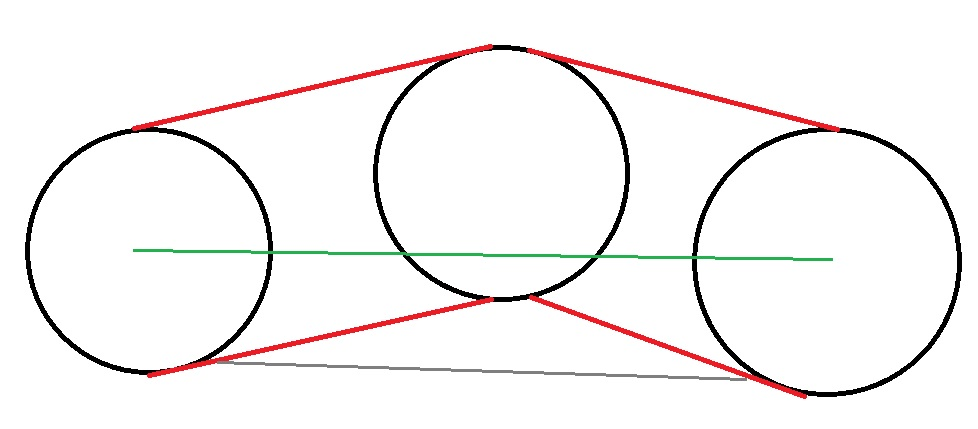
\includegraphics[height=3in]{hw1prob1-10b_1.jpg}
\caption{In Red is the straight line part of the hull, Black is the circles. The gray line shows the violation of convexity}
\end{figure}
In the case where the center of the circle is on the line from the left-most point to right-most point, the convex hull will only cover two points on the circle and will thus still be straight lines and not consist of the boundary.
\begin{figure}[H]
\centering
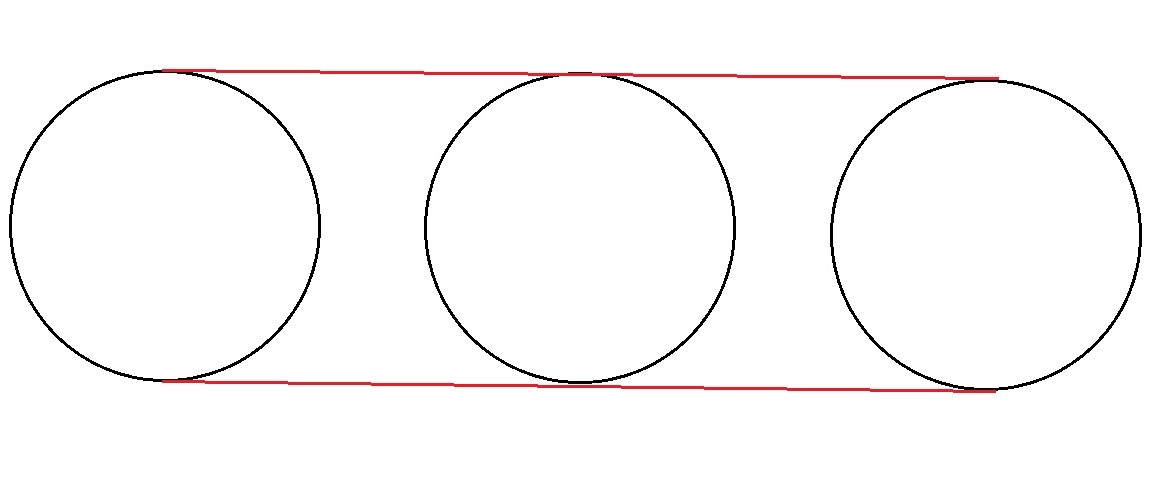
\includegraphics[height=3in]{hw1prob1-10b_2.jpg}
\caption{In Red is the straight line part of the hull, Black is the circles.}
\end{figure}
Since we have a contradiction for both cases where a convex hull appears in two different places on the boundary of a circle, it is impossible for that to occur, thus the convex hull is either on the boundary once or not at all. 

\subsection*{Problem 1.10c}

For the forward proof, assume that a point p is in convex hull of S' but the corresponding circle p* is not in the convex hull of S. 
\\This means that p* must lie inside the convex hull of S. 
\\Take the circles $q_1*,...,q_n*$ on the convex hull boundary and let $q_1,...,q_n$ be the corresponding centers. 
\\Since all the circles have equal radii, this means that p will be inside the polygon $q_1,...,q_n$ \\
However p is on the convex hull, so this violates convexity. This is a contradiction.\\
\\
For the backward proof, assume that a circle p* is in the convex hull of S but the corresponding center p is not in the convex hull of S'. \\
This means that p must lie inside the convex hull of S'.
\\Take the circle centers $q_1,...,q_n$ on the convex hull of S and let $q_1*,...,q_n*$ be the corresponding circles.
\\Since all the circles have equal radii, this means that p* will be inside the polygon formed by $q_1,...,q_n*$\\
However, p* is on the convex hull, so this violates convexity, leading to a contradiction. 

\subsection*{Problem 1.10d}

The idea of the algorithm is that we will find the convex hull of the centers and then use that to get the total convex hull. Here is the algorithm:\\
1. Find the convex hull of the centers\\
2. For every line pq in that convex hull\\
			Find line perpendicular to pq that passes through p and line perpendicular to pq that passes through q, call them p1 and q1\\
			Find the intersections of the p circle with p1 and intersections of q circle with q1, call them p1*, p2*, q1*, q2*. Make sure p1*, q1* are on the same side of the pq line segment. \\
			If there are only two circles, then connect p1* and q1* in one segment and then p2* and q2* in another segment. The hull is then p1*,q1*,q2*,p2*,p1*\\
			If there are more than two circles, then make p1*,q1* the pair that outside the convex hull of the centers. Connect p1* and q1* and make that part of the hull\\
3. You now have circles and straight lines. Travel along the straight lines and add it to hull. When you reach a circle, you have to decide which part of the boundary to add to the hull\\
			-Add the part of that circle that will make slope decrease if doing the upper hull.\\
			-Add the part to make the slope increase if doing the lower hull.

\subsection*{Problem 1.10e}

This algorithm will build up the hull circle by circle.\\
1. Initialize hull H with circle 1
2. For each circle C\\
	- Find the center of hull H and call it h. Can be done by getting the center of the left-most, right-most, upper-most and lower-most points on the hull. \\
	- Call the center of the circle c. \\
	- Find the lines $H_1$ and $H_2$ that are tangent to the hull and perpendicular to the line formed by hc. \\
	- Find the lines $C_1$ and $C_2$ that are tangent to the circle and perpendicular to the line formed by hc. \\
	- Search the tangent lines from $H_1$ to $H_2$ until you find one that goes through $C_1$ and $C_2$ and touches the circle once. Add that line to the hull H. \\
	- Repeat above step for tangent lines from $H_2$ to $H_1$. 
	- Add the arc in the circle between those lines to the hull H\\
\begin{figure}[H]
\centering
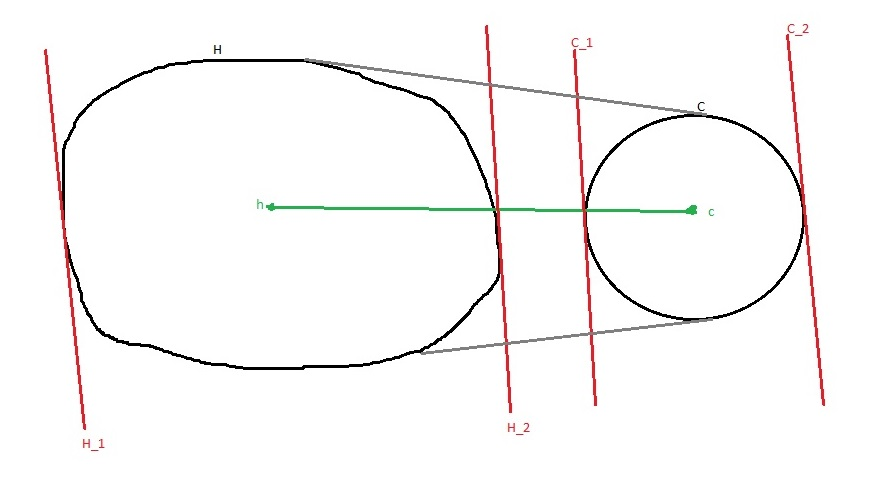
\includegraphics[height=4in]{hw1prob1-10e.jpg}
\caption{Illustration of the above parts. The gray lines are the parts of the hull that get added}
\end{figure}
Correctness:\\
At each step, we are making sure to add the necessary part of the circle and we are also ensuring convexity.\\
\\
Run-time:\\
The loops is run on the n circles. \\
For each circle, there is a constant number of operations except for the searching. \\
The searching can be done in $log(n)$ time by using a binary search tree to implement it. \\
The total run time is thus $O(n log(n) )$
\newpage

\section*{Problem 8.2}

\subsection*{Problem 8.2a}

The dual of a collection of points inside a triangle with vertices p,q,r will be a collection of lines from the union of the double wedges for pq, qr, and pr. 
\\
When you take $p*, q*, r*$, the division of the plane forms 6 wedges. There are 7 faces when you include the inner triangle formed. In the following figure the dual ends up being everything except section 5 and 6. It will end up looking like a double wedge with an extra triangle in the middle. 

\begin{figure}[H]
\centering
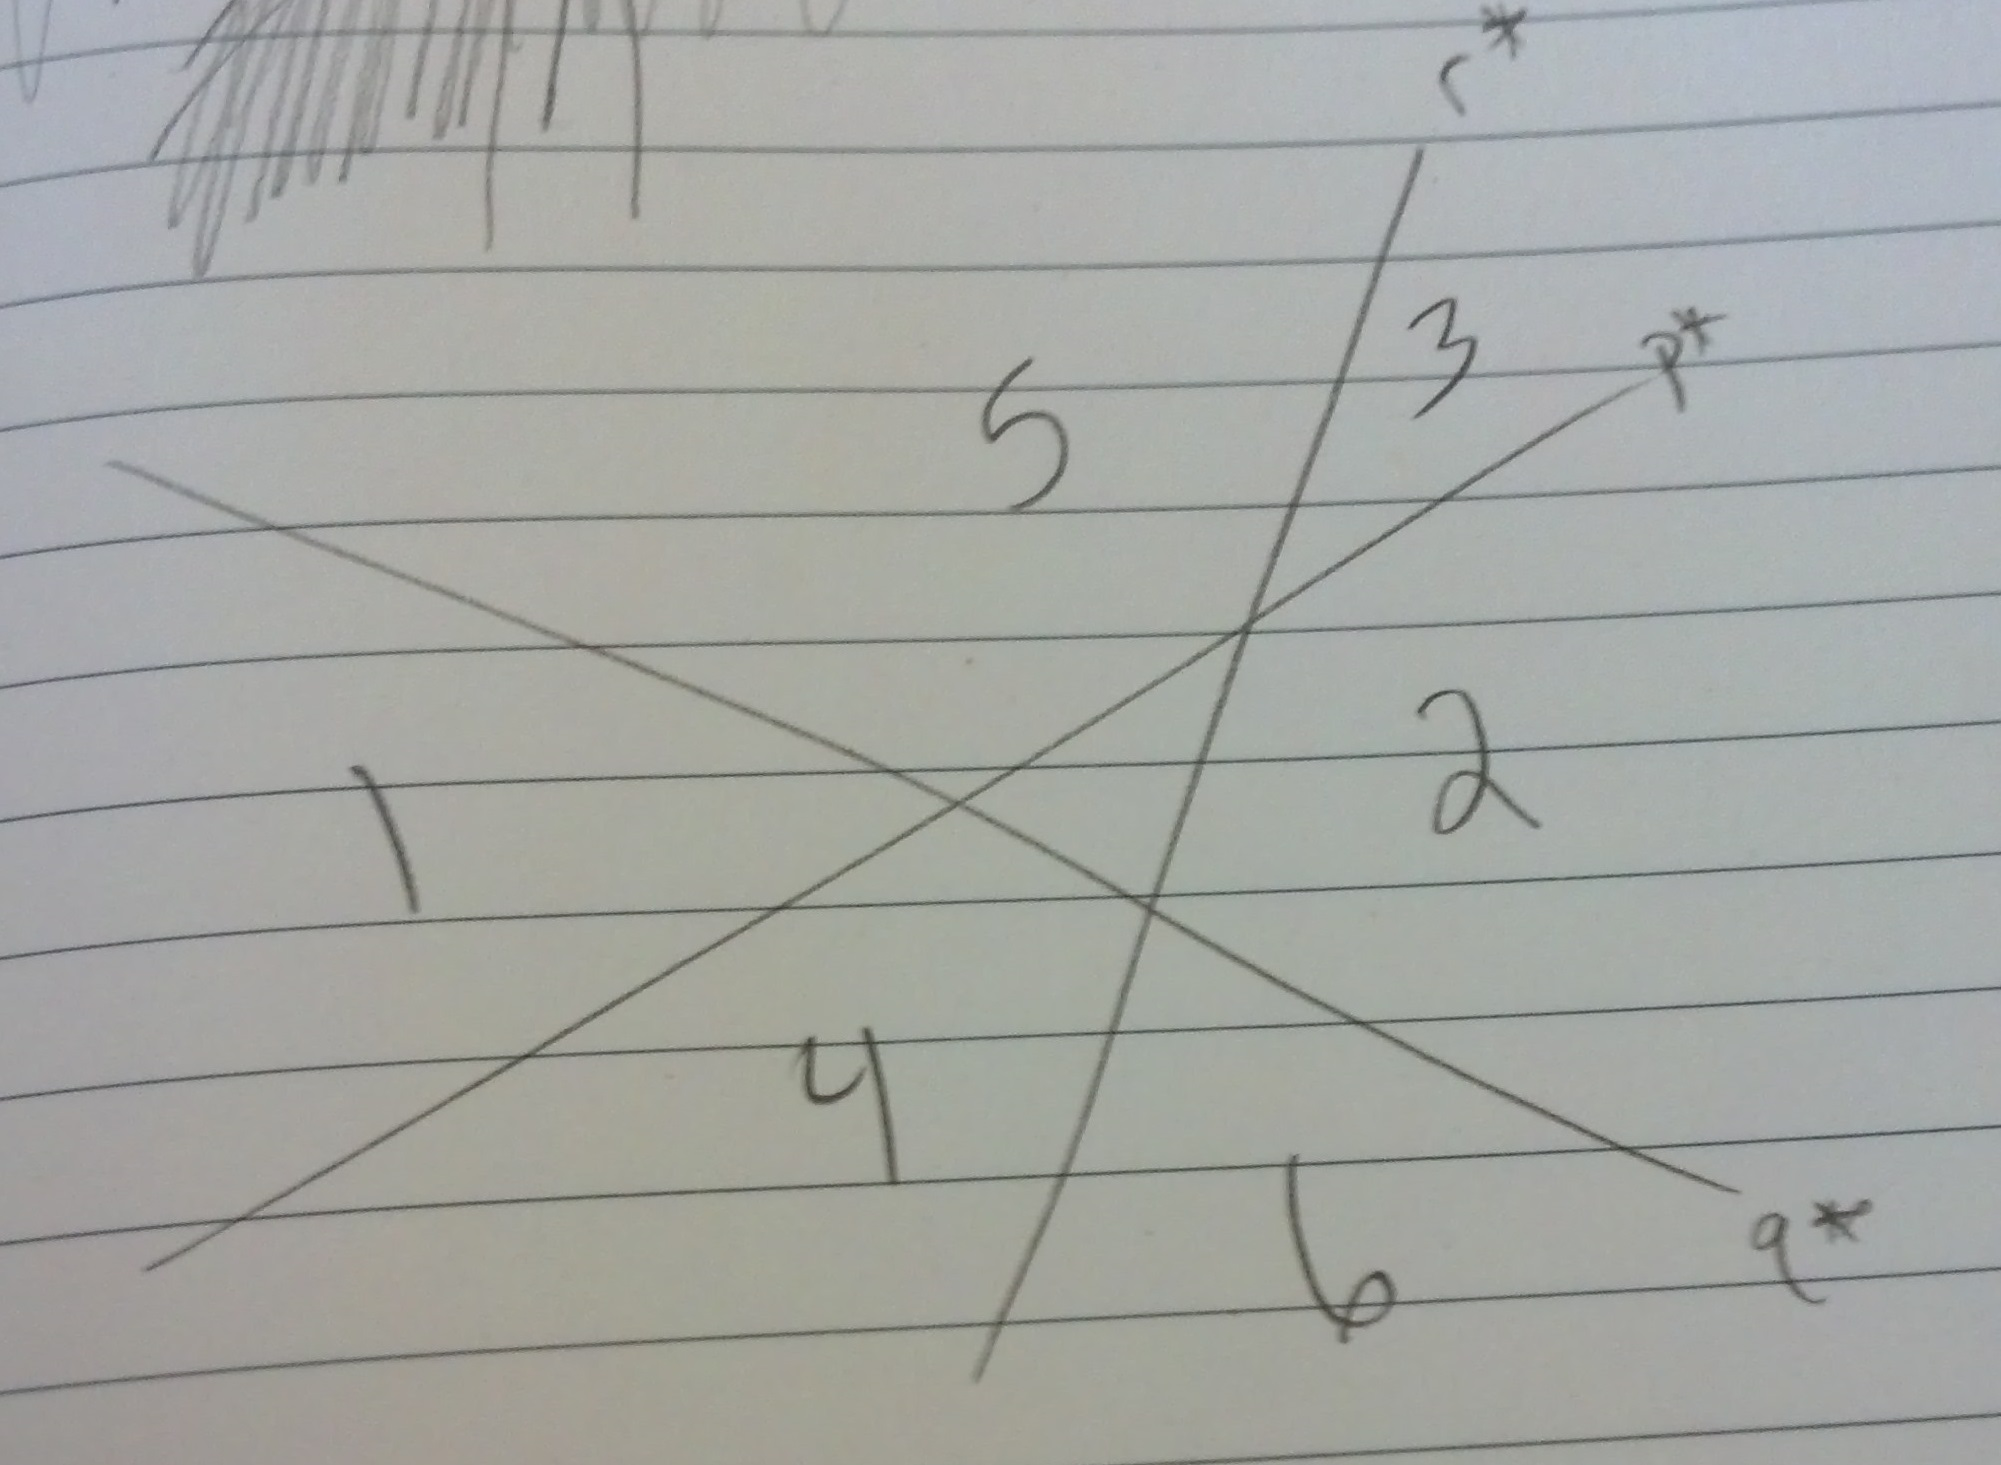
\includegraphics[height=4in]{cs266dual.jpg}
\caption{Illustration of the wedges}
\end{figure}

\newpage

\subsection*{Problem 8.2b}

In the illustration, the left-right double wedge is formed by the line segment. The dual lines all meet in that point since the primal points are co-linear. If we take the entire line formed by pq, the dual of that is the union of all lines that pass through that point. For the top-bottom double wedge, we would then want that whole union minus the left-right double wedge. \\
\\
A line segment $pq$ can be described as $\{tp + (1-t)q\}$ for $0 \leq t \leq 1$. The two rays we want whose dual is a top-bottom double wedge will be the whole line minus that segment thus it is $\{tp + (1-t)q\}$ for $t < 0$ and $t > 1$. 

\section*{Problem 8.6}

The duality transform is incidence-preserving thus the dual of the problem is whether any of the m points in the dual of L lie on any of the n lines in the dual of S. 


\end{document}








